\documentclass{article}
\usepackage{tikz, comment}
\usepackage{pifont}
\usepackage{fontspec, pgfplots}
\usetikzlibrary{arrows, decorations.markings, decorations.pathreplacing}
\begin{comment}
:Title: Not defined yet
:Tags: directrices of a hyperbola;focus of a parabola;moment;directrix of a parabola;median of a trapezoid
:Prob: 0.5487;0.5409;0.5402;0.5294;0.5243
:Author: Prof.Hu Ji-shan, HKUST
:Slug: No name yet

Description Here.........
\end{comment}
\begin{document}\centering 

\pgfplotsset{
    colormap/outside/.style={
        colormap=
            {outside}{
            rgb255(0cm)=(110,110,255);
            rgb255(1cm)=(20,20,255);
            }
    },
    colormap/outside,
    colormap/inside/.style={
        colormap={inside}{
            rgb255(0cm)=(20,20,255);
            rgb255(1cm)=(220,220,255);
        }
    },
    colormap/inside
}

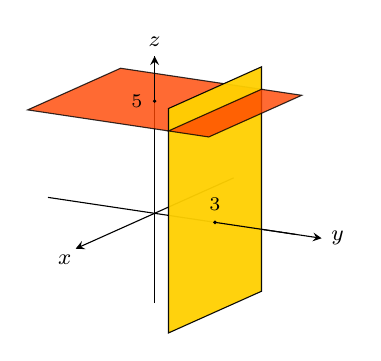
\begin{tikzpicture}[font=\footnotesize]
\begin{axis}
[axis lines = center, view={120}{15}, scale=0.8, ticks=none,
axis background, xlabel = {$x$}, ylabel ={$y$}, zlabel ={$z$}, domain =-2:2, y domain =-2:2,
samples =20, samples y =40, z buffer = auto, 
axis equal, 
%xmin=0, xmax=8,
%ymin=-4, ymax=4,
zmin=-4, zmax=7,
every axis x label/.style={
    at={(ticklabel* cs:1)},
    anchor= east, xshift = 2, yshift=-4
},
every axis y label/.style={
    at={(ticklabel* cs:1)},
    anchor= west, 
},
every axis z label/.style={
    at={(ticklabel* cs:1)},
    anchor= south
}]

    \addplot3 [
      surf, 
      domain=-4:4,
      samples=2,
      y domain=-4:3,
      samples y=2,
%      line join=round,  
      shader=interp,
%      mesh/interior colormap name=inside,
%      colormap/outside,
      shader=faceted,
      variable=\t,
%      point meta={t},
      faceted color=black, opacity=0.8
    ]
           ({t},{y},{5});


    \addplot3 [
      surf,
      domain=-4:4,
      samples=2,
      y domain=-4:6,
      samples y=2,
%      line join=round,  
      shader=interp,
%      mesh/interior colormap name=inside,
%      colormap/outside,
      shader=faceted,
      variable=\t,
%      point meta={t},
      faceted color=black, opacity=0.95
    ]
           ({t},{3},{y});

    \addplot3 [
      surf, 
      domain=-4:4,
      samples=2,
      y domain=3:5,
      samples y=2,
%      line join=round,  
      shader=interp,
%      mesh/interior colormap name=inside,
%      colormap/outside,
      shader=faceted,
      variable=\t,
%      point meta={t},
      faceted color=black, opacity=0.8
    ]
           ({t},{y},{5});

    \addplot3 [
      surf, black,
      domain=5:7,
      samples=2,
      y domain=0:0,
      samples y=2,
%      line join=round,  
      shader=interp,
%      mesh/interior colormap name=inside,
%      colormap/outside,
      shader=faceted,
      variable=\t,
%      point meta={t},
      faceted color=black, opacity=1
    ]
           ({0},{0},{t});
           
    \addplot3 [
      surf, black,
      domain=3:7,
      samples=2,
      y domain=0:0,
      samples y=2,
%      line join=round,  
      shader=interp,
%      mesh/interior colormap name=inside,
%      colormap/outside,
      shader=faceted,
      variable=\t,
%      point meta={t},
      faceted color=black, opacity=1
    ]
           ({0},{t},{0});
                                         
\node[label={180:{\scriptsize $5$}},circle,fill,inner sep=0.5pt] at (axis cs:0,0,5) {};
\node[label={90:{\scriptsize $3$}},circle,fill,inner sep=0.5pt] at (axis cs:0,3,0) {};

\end{axis}

\end{tikzpicture}
\end{document}